\documentclass{beamer}
\usepackage{amsmath}
\usepackage{graphicx}
\begin{document}
\begin{frame}
  \frametitle{Numerical Analysis Using Finite Difference Method}
    \begin{center}
    \Large{GROUP 6}
  \end{center}
 
  \vspace{1cm}
  
 
  \begin{itemize}
    \item Eric Kazungu SCT211-0028/2021
    \item Samuel Wainaina SCT211-0039/2021
    \item Keith Kareithi SCT211-0021/2021
  \end{itemize}
  
\end{frame}

\begin{frame}
\frametitle{Introduction}

This method is used to find the solution to differential equations including partial differential equations. This means that given a function's derivatives, we can obtain the original function numerically using this method. 

\pause

This method actually stems from the very first idea we learned when dealing with differentiation where we use it to find the derivative of a function. Given a sufficiently smooth function $f(x)$, the derivative of $f$ is defined as

\[
f'(x) = \lim_{h\to 0} \frac{f(x+h) - f(x)}{h}.
\]

\pause

For instance, if the point is 2 in the curve we can pick point $f(x + h) = f(3)$. In this, we can calculate the gradient as $y_x$ where a change in $y$ is $f(3) - f(2)$ and change in $x$ is $h$. In this case, the gradient from this calculation is a very bad estimate, however, this estimate gets better as $h$ gets smaller and smaller. This is the basis for the finite difference method.

\end{frame}

\begin{frame}
\frametitle{The Three Types of Finite Difference Methods}

With this in mind, we can also say that there are two other possibilities. The first one we just went through in the introduction is called the Forward Difference Method. The others are the following:

\begin{enumerate}
\item Backward difference method: In this case, we use the value behind the chosen point to find the value of $f'(x)$:
\[
f'(x) = \frac{f(x) - f(x-h)}{h}.
\]

\item Central difference method: This is the interesting one amongst the three because it can easily help us find the second derivative of $f(x)$. In this case, we use the 2 points on the adjacent sides of our chosen point $f(x)$ to find $f'(x)$:
\[
f'(x) = \frac{f(x+h) - f(x-h)}{2h}.
\]
\end{enumerate}

\end{frame}
\begin{frame}{Second derivative using central difference method}
In order to find the second derivative using central difference method, we need the point between $f(x+h)$ and $f(x)$ as well as the point between $f(x-h)$ and $f(x)$ and find the gradient for them using the central difference method, i.e.,

\[f'(x+\frac{1}{2}h) &= \frac{f(x+h) - f(x)}{h}\]
\[f'(x-\frac{1}{2}h) &= \frac{f(x) - f(x-h)}{h}\]

\end{frame}
\begin{frame}{Second derivative using central difference method}
Then apply the method again to these two gradients to find $f''(x)$:


\[f''(x) &= \frac{f'(x+\frac{1}{2}h) - f'(x-\frac{1}{2}h)}{h}\] 
\[&=\frac{\frac{f(x+h) - f(x)}{h} - \frac{f(x) - f(x-h)}{h}}{h}\] 
\[&=\frac{f(x+h) + f(x-h) - 2f(x)}{h^2}\]


In this form, we have a very powerful equation that can help us find the second derivative of a function.
\end{frame}

\begin{frame}{Integration using central difference method}
By simply rearranging the equations from the central difference method to make $f(x)$ the subject of the formula, we can derive the original function numerically using the derivatives. This means that we can use the central difference method to find the solution to a differential equation.

For example, consider the second derivative formula we derived using the central difference method:

\begin{equation*}
f''(x) = \frac{f(x+h) + f(x-h) - 2f(x)}{h^2}
\end{equation*}

We can rearrange this formula to solve for $f(x)$ as:

\begin{equation*}
f(x) = \frac{1}{2}(f(x+h) + f(x-h) - h^2f''(x))
\end{equation*}

Using this formula, we can numerically compute the value of $f(x)$ for any given $x$, using the values of $f(x\pm h)$ and $f''(x)$.

\end{frame}
\begin{frame}{Algorithm}
\begin{enumerate}
\item Set the boundaries and conditions which are the maximum iterations($N$),
the step size($h$), the lower limit(LL), and the upper limit(UL).
\item Define the function $f(x)$.
\item Define the second-order derivative for the function, denoted as $f''(x)$.
\item Get the values of $f(UL)$ and $f(LL)$ and use them to calculate the gradient
$\frac{f(UL)-f(LL)}{UL-LL}$.
\item Create a list of elements within the range of [LL, UL] in intervals of $h$.
\item For each element $x$ in the list obtained in step 5, determine the value of $y$
by multiplying $x$ with the gradient obtained in step 4.
\item For each point $(x, y)$ obtained in step 6, use the formula $f(x) = f(x + h) + f(x - h) - f''(x)h$
substituting $f''(x)$ with the defined differential equation to calculate the approximate values of $f(x)$ for the solution to the differential equation.
\item Plot these approximate values alongside the graph of the exact function $f(x)$ to validate the accuracy of the code.
\end{enumerate}
\end{frame}

\begin{frame}{Example: Central Difference Method}
    Consider the second derivative function:
    $$\frac{d^2 f}{dx^2} = x^2 - 2$$
    The range is from 0 to 3 as shown below:
    $$f(0) = 0, \quad f(3) = 2$$
    The Central Finite's method second derivative is:
    $$f''(x) = f(x + h) + f(x - h) - 2f(x){h^2}$$
    And as it is the second derivative, it is also equal to:
    $$f''(x) = x^2 - 2$$
    As a result, we have:
    $$f''(x) = x^2 - 2 = f(x + h) + f(x - h) - 2f(x){h^2}$$
\end{frame}
\begin{frame}{Example}


When we rearrange the equation and do some calculations we get,

$$f(x + h) + f(x - h) - 2f(x) = (x^2 - 2)h^2$$ \\

$$2f(x) = f(x + h) + f(x - h) - \frac{(x^2 - 2)h^2}{2}$$

Finally, we get $f(x)$ as shown below,

$$f(x) =\frac{ f(x+h) + f(x-h) - f''(x)h^2}{2}$$

\end{frame}

\begin{frame}[fragile]{Iterative Solution of a Differential Equation}
\begin{verbatim}
import numpy as np
import matplotlib.pyplot as plt

# Define functions
def diff2_central(f, x, h=0.1):
    return (f(x+h)-2*f(x)+f(x-h))/h**2

def exact_func(x):
    C = (11-81/12)/3
    return x*4/12 - x*2 + C*x

def fn(x):
    return x**2 - 2
\end{verbatim}
\end{frame}
\begin{frame}[fragile]{Iterative Solution of a Differential Equation}
\begin{verbatim}
# Set up the graph for the exact function
fig, ax = plt.subplots()
ax.set_xlabel('x')
ax.set_ylabel('y')
ax.set_xlim(0, 3)
ax.set_ylim(0, 3)

# Plot the initial function f(x)
dx = 0.01
x = np.arange(0, 3, dx)
y = exact_func(x)
ax.plot(x, y, color='red')

\end{verbatim}
\end{frame}
\begin{frame}[fragile]{Iterative Solution of a Differential Equation}
\begin{verbatim}
# Define variables and initial conditions
z = 3  # higher limit range
x = 0  # lower limit range
h = 0.2  # step size
xp = np.arange(0, 3+h, h)
m = exact_func(z)/abs(z-x)
fp = m*xp
fp2 = m*xp
colors = ['purple', 'yellow', 'cyan', 'green']


# Plot the initial function fp(x)
ax.plot(xp, fp, color='blue', marker='o')

\end{verbatim}
\end{frame}
\begin{frame}[fragile]{Iterative Solution of a Differential Equation}
\begin{verbatim}
# Iteratively update the function fp(x)
N = 200
for n in range(N):
    fdata = []
    for i in range(1, len(xp)-1):
        fp2[i] = 0.5*(fp[i+1]+fp[i-1]-h*2(fn(xp[i])))

    for i in range(len(xp)):
        fp[i] = fp2[i]
        fdata.append([xp[i], fp[i]])

    # Update the plot every 50 iterations
    if n % 50 == 0:
        color_index = n // 50 % len(colors)
        ax.plot(xp, fp, color=colors[color_index], marker='o')

plt.show()
\end{verbatim}
\end{frame}
\begin{frame}
  \frametitle{Result}
  \begin{center}
    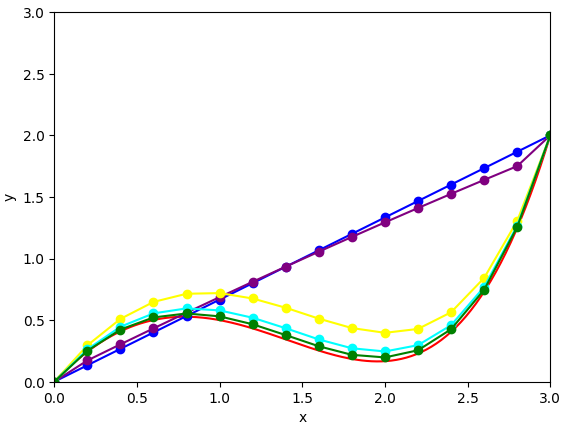
\includegraphics[width=1.0\textwidth]{graph.png}
  \end{center}
\end{frame}

\begin{frame}{Conclusion}
The finite difference method is a powerful technique for solving a wide range
of problems in numerical analysis. In this article, we have seen how it can be
applied to the solution of differential equations where we can use finite difference
formulas to approximate derivatives.
\end{frame}
\end{document}